\documentclass[hidelinks,11pt,dvipsnames]{article}
% xcolor commonly causes option clashes, this fixes that
\PassOptionsToPackage{dvipsnames,table}{xcolor}
\usepackage[tmargin=1in, bmargin=1in, lmargin=0.8in, rmargin=1in]{geometry}

%%%%%%%%%%%%%%%%%%%%%%%%%%%%%%%%%%%%%%%%%%%%%%%%%%%%%%%%%%%%%%%%%%%%
%%% For inkscape-figures
%%% Assumes the following directory structure:
%%% master.tex
%%% figures/
%%%     figure1.pdf_tex
%%%     figure1.svg
%%%     figure1.pdf
%%%%%%%%%%%%%%%%%%%%%%%%%%%%%%%%%%%%%%%%%%%%%%%%%%%%%%%%%%%%%%%%%%%%
%\usepackage{import}
\usepackage{pdfpages}
\usepackage{transparent}

\newcommand{\incfig}[2][1]{%
    \def\svgwidth{#1\columnwidth}
    \import{./figures/}{#2.pdf_tex}
}

\pdfsuppresswarningpagegroup=1

% enable synctex for inverse search, whatever synctex is
\synctex=1
\usepackage{float,macrosabound,homework,theorem-env}
\usepackage{microtype}


% font stuff
\usepackage{sectsty}
\allsectionsfont{\sffamily}
\linespread{1.1}

% bibtex stuff
\usepackage[backend=biber,style=alphabetic,sorting=anyt]{biblatex}
\addbibresource{main.bib}

% colored text shortcuts
\newcommand{\blue}[1]{\color{MidnightBlue}{#1}}
\newcommand{\red}[1]{\textcolor{Mahogany}{#1}}
\newcommand{\green}[1]{\textcolor{ForestGreen}{#1}}


% use mathptmx pkg while using default mathcal font
\DeclareMathAlphabet{\mathcal}{OMS}{cmsy}{m}{n}

% fixes the positioning of subscripts in $$ $$
\renewcommand{\det}{\operatorname{det}}

\usetikzlibrary{positioning, arrows.meta}
\newcommand{\here}[2]{\tikz[remember picture]{\node[inner sep=0](#2){#1}}}

%%%%%%%%%%%%%%%%%%%%%%%%%%%%%%%%%%%%%%%%%%%%%%%%%%%%%%%%%%%%%%%%%%%%%
%%% Entry Counter
%%%%%%%%%%%%%%%%%%%%%%%%%%%%%%%%%%%%%%%%%%%%%%%%%%%%%%%%%%%%%%%%%%%%%
\newcounter{entry-counter}
\newcommand{\entry}[1]
{
	\addtocounter{entry-counter}{1}
    \tchap{Entry \arabic{entry-counter}}
	%\addcontentsline{toc}{section}{Entry \arabic{entry-counter}: #1}
	\vspace{-1.5em}
    \begin{center}
		\small \emph{Written: #1}
    \end{center}
}

\usepackage{titling}
\renewcommand\maketitlehooka{\null\mbox{}\vfill}
\renewcommand\maketitlehookd{\vfill\null}


\usepackage{capt-of}
\usepackage{tikz}
\usepackage{listings}
\usetikzlibrary{positioning,calc,intersections,through,backgrounds, shapes.geometric, decorations.markings,arrows}

\def\sset{\subseteq}
\def\iso{\cong}
\def\gend#1{\langle #1\rangle}

\newcommand{\rightoverleftarrow}{%
  \mathrel{\vcenter{\mathsurround0pt
    \ialign{##\crcr
      \noalign{\nointerlineskip}$\longrightarrow$\crcr
      \noalign{\nointerlineskip}$\longleftarrow$\crcr
    }%
  }}%
}

\newcommand\makesphere{} % just for safety
\def\makesphere(#1)(#2)[#3][#4]{%
  % Synopsis
  % \makesphere[draw options](center)(initial angle:final angle:radius)
  \shade[ball color = #3, opacity = #4] #1 circle (#2);
  \draw #1 circle (#2);
  \draw ($#1 - (#2, 0)$) arc (180:360:#2 and 3*#2/10);
  \draw[dashed] ($#1 + (#2, 0)$) arc (0:180:#2 and 3*#2/10);
}
% same thing as makesphere but places white background behind
\newcommand\altmakesphere{} % just for safety
\def\altmakesphere(#1)(#2)(#3)[#4][#5]{%
  % Synopsis
  % \make sphere[draw options](center)(initial angle:final angle:radius)
  \draw [fill=white!30] #1 circle (#2);
  \shade[ball color = #4, opacity = #5] #1 circle (#2);
  \draw #1 circle (#2);
  \draw ($#1 - (#2, 0)$) arc (180:360:#2 and 3*#2/10);
  \draw[dashed] ($#1 + (#2, 0)$) arc (0:180:#2 and 3*#2/10);
  \node at #1 {#3};
}

\begin{document}
% set section number to 1
% fixes theorem numbering without need to have a section title
\setcounter{section}{1}

\pagestyle{empty}
	\LARGE
\begin{center}
	Foundations of Data Science and Machine Learning -- \emph{Homework 2}\\
	\Large
	Isaac Martin \\
    Last compiled \today
\end{center}
\normalsize
\vspace{-4mm}
\hru

\begin{homework}[e]
  \prob In $d$-dimensions there are at most $d$ unit vectors that are pairwise orthogonal. However, if you wanted a set of vectors that were ``almost orthogonal'' you might squeeze in a few more. For example, in 2-dimensions if you wanted vectors at least 45 degrees apart, then you could fit in three vectors. Suppose you wanted to find $1000$ almost orthogonal vectors in 100 dimensions. Here are two ways you could try doing it:
  \begin{enumerate}[(a)]
    \item Begin with 1000 orthonormal 1000-dimensional vectors, and then project them to a random $100$-dimensional space.
    \item Generate $1000$ 100-dimensional random standard Gaussian vectors.
  \end{enumerate}
  \begin{soln}$ $
    \begin{enumerate}[(a)]
      \item We generated 1000 1000-dimensional standard Gaussian vectors, stuck these in the columns of a matrix $A$ and then performed QR-factorization to extract out the orthonormal basis for the span of $A$. The probability of choosing $1000$ vectors which are linearly dependent in $\bR^{1000}$ ought to be zero -- if you have chosen $k < 1000$ vectors already then the $k$-dimensional subspace spanned by these vectors has measure zero in $\bR^n$ -- but we check that the determinant of $Q$ is not zero before proceeding.

        As an aside: rather than fixing a random 100-dimensional subspace, we simply project the columns of $Q$ to the subspace spanned by $e_1,...,e_{100}$. This is actually equivalent to projecting to a random 100-dimensional subspace. Any two $d$-dimensional linear subspaces of $\bR^{n}$ are related by the action of $O(n)$, that is, if $V,W \subseteq \bR^n$ are linear subspaces then there is some $P \in O(n)$ such that $P \cdot V = W$. Furthermore, $P$ is an isometry of $\bR^n$, meaning for any $u,v \in \bR^n$, $\langle u,v \rangle = \langle Pu,Pv \rangle$. We're using ``the closeness of the dot product to zero'' as our measure of ``orthogonal-ness'', so we might as well take the dot product in $\spann_\bR\{e_1,...,e_{100}\}$ to make the projection easier.

        We now project the columns of $Q$ to the subspace spanned by $e_1,...,e_{100}$, i.e. we truncate the 900 tail components from each column of $Q$. At this point, we would like to take the pairwise dot product of distinct columns and examine the results. However, the projection $\bR^{1000} \to \bR^{100}$ results in a large loss of norm, and because we will be comparing this process to Gaussian sampling in part (b), we renormalize our vectors to ensure that the magnitude of our dot product solely reflects the angle between the vectors.

        The results of this process can be seen in the ``discussion'' section.

      \item For method b, we generated 1000 100-dimensiona iid standard Gaussian vectors and normalized them before calculating the pairwise dot products of distinct vectors. This was more straightforward than method 2 as it doesn't involve projecting to a lower dimensional vector space.
    \end{enumerate}

    \emph{Discussion.} ~ Here are histograms illustrating the results methods (a) and (b).
    \begin{center}
      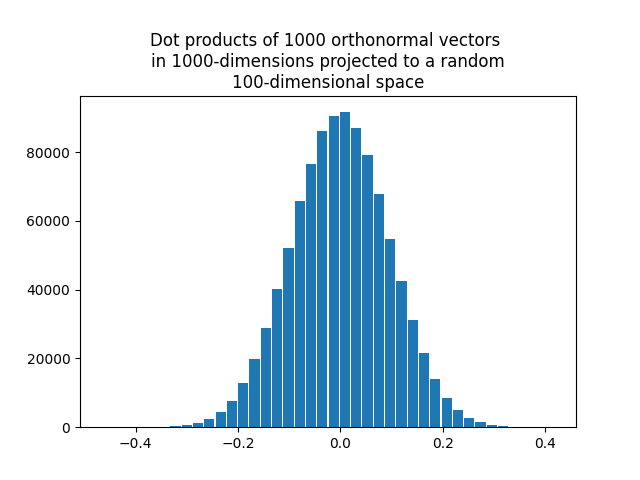
\includegraphics[width=12cm]{~/Desktop/university/code/dsml/hwk2/prob1a.png}
      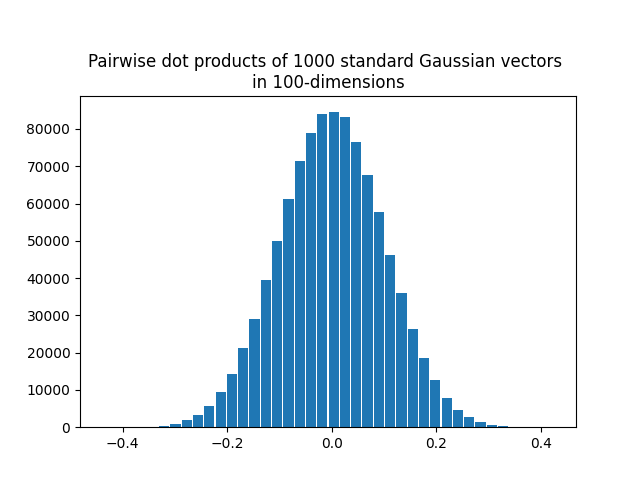
\includegraphics[width=12cm]{~/Desktop/university/code/dsml/hwk2/prob1b.png}
      \captionof{figure}{Density of pairwise dot product values for the two ``almost orthogonal'' methods}
      \label{fig:prob1}
    \end{center}
    As you can see, the two methods produced similar results. Neither produced dot product values outside of $[-0.35,0.35]$, and hence no two vectors were closer than $\cos^{-1}(0.35) = 70^\circ$ apart. The second method was marginally worse, as it has a slightly flatter density curve.
  \end{soln}
  \prob$ $
  \begin{enumerate}[(a)]
    \item Fix $\bfx, \bfy \in \bR^d$ both with an $\ell_2$-norm of 1. Suppose that $\Phi:\bR^d\to \bR^r$ is a linear map satisfying
      \begin{equation}\label{eqn:2.1}
        (1  - \epsilon)\|\bfx + \bfy\|_2^2 \leq \|\Phi(\bfx + \bfy)\|^2_2 \leq (1+\epsilon)\|\bfx + \bfy\|^2_2
      \end{equation}
      and
      \begin{equation}\label{eqn:2.2}
        (1  - \epsilon)\|\bfx - \bfy\|_2^2 \leq \|\Phi(\bfx - \bfy)\|^2_2 \leq (1+\epsilon)\|\bfx - \bfy\|^2_2.
      \end{equation}
      Use the identity $4\langle \bfu, \bfv \rangle = \|\bfu + \bfv\|^2_2 - \|\bfu-\bfv\|^2_2$ to show that
      \begin{align*}
        \left|\langle \bfx,\bfy \rangle - \langle \Phi(\bfx),\Phi(\bfy) \rangle \right|\leq \epsilon\|\bfx\|_2\|\bfy\|_2.
      \end{align*}
    \item If $\chi = \{\bfx_1,...,\bfx_n\}$ is an arbitrary fixed set in $\bR^d$ and $\Phi:\bR^d \to \bR^r$ is a random matrix with independent mean-zero variance $1/r$ Gaussian entries, how should the embedding dimension $r$ scale in terms of $n$, $d$, $\epsilon$ so that with probability at least $0.9$ it holds
      \begin{align*}
        |\langle \bfx_j,\bfx_k \rangle - \langle \Phi(\bfx_j),\Phi(\bfx_k) \rangle| \leq \epsilon \|\bfx_j\|_2\|\bfx_k\|_2.
      \end{align*}
  \end{enumerate}
  \begin{prf}$ $
    \begin{enumerate}[(a)]
      \item Rearrange both equation (\ref{eqn:2.1}) and (\ref{eqn:2.2}) as follows:
        \begin{equation}\label{eqn:2.3}
          -\epsilon\|\bfx +\bfy\|_2^2 \leq \|\Phi(\bfx + \bfy)\|_2^2 - \|\bfx + \bfy\|_2^2 \leq \epsilon\|\bfx + \bfy\|^2_2
        \end{equation}
        \begin{equation}\label{eqn:2.4}
          -\epsilon\|\bfx -\bfy\|_2^2 \leq \|\Phi(\bfx - \bfy)\|_2^2 - \|\bfx - \bfy\|_2^2 \leq \epsilon\|\bfx - \bfy\|^2_2.
        \end{equation}
        Adding equation (\ref{eqn:2.4}) to the negative of (\ref{eqn:2.3}) yields
        \begin{align*} 
          -\epsilon(\|\bfx + \bfy\|^2_2 + \|\bfx - \bfy\|^2_2) \leq \|\bfx + \bfy\|^2_2 &- \|\bfx - \bfy\|_2^2 - (\|\Phi(x + y)\|^2_2 - \|\Phi(x - y)\|^2_2)\\
          &\leq \epsilon(\|\bfx + \bfy\|^2_2 + \|\bfx - \bfy\|^2_2).
        \end{align*}
        Let's examine the term $\|\bfx + \bfy\|^2_2 + \|\bfx - \bfy\|^2_2$. Consider the following illustration:
        \begin{center}
          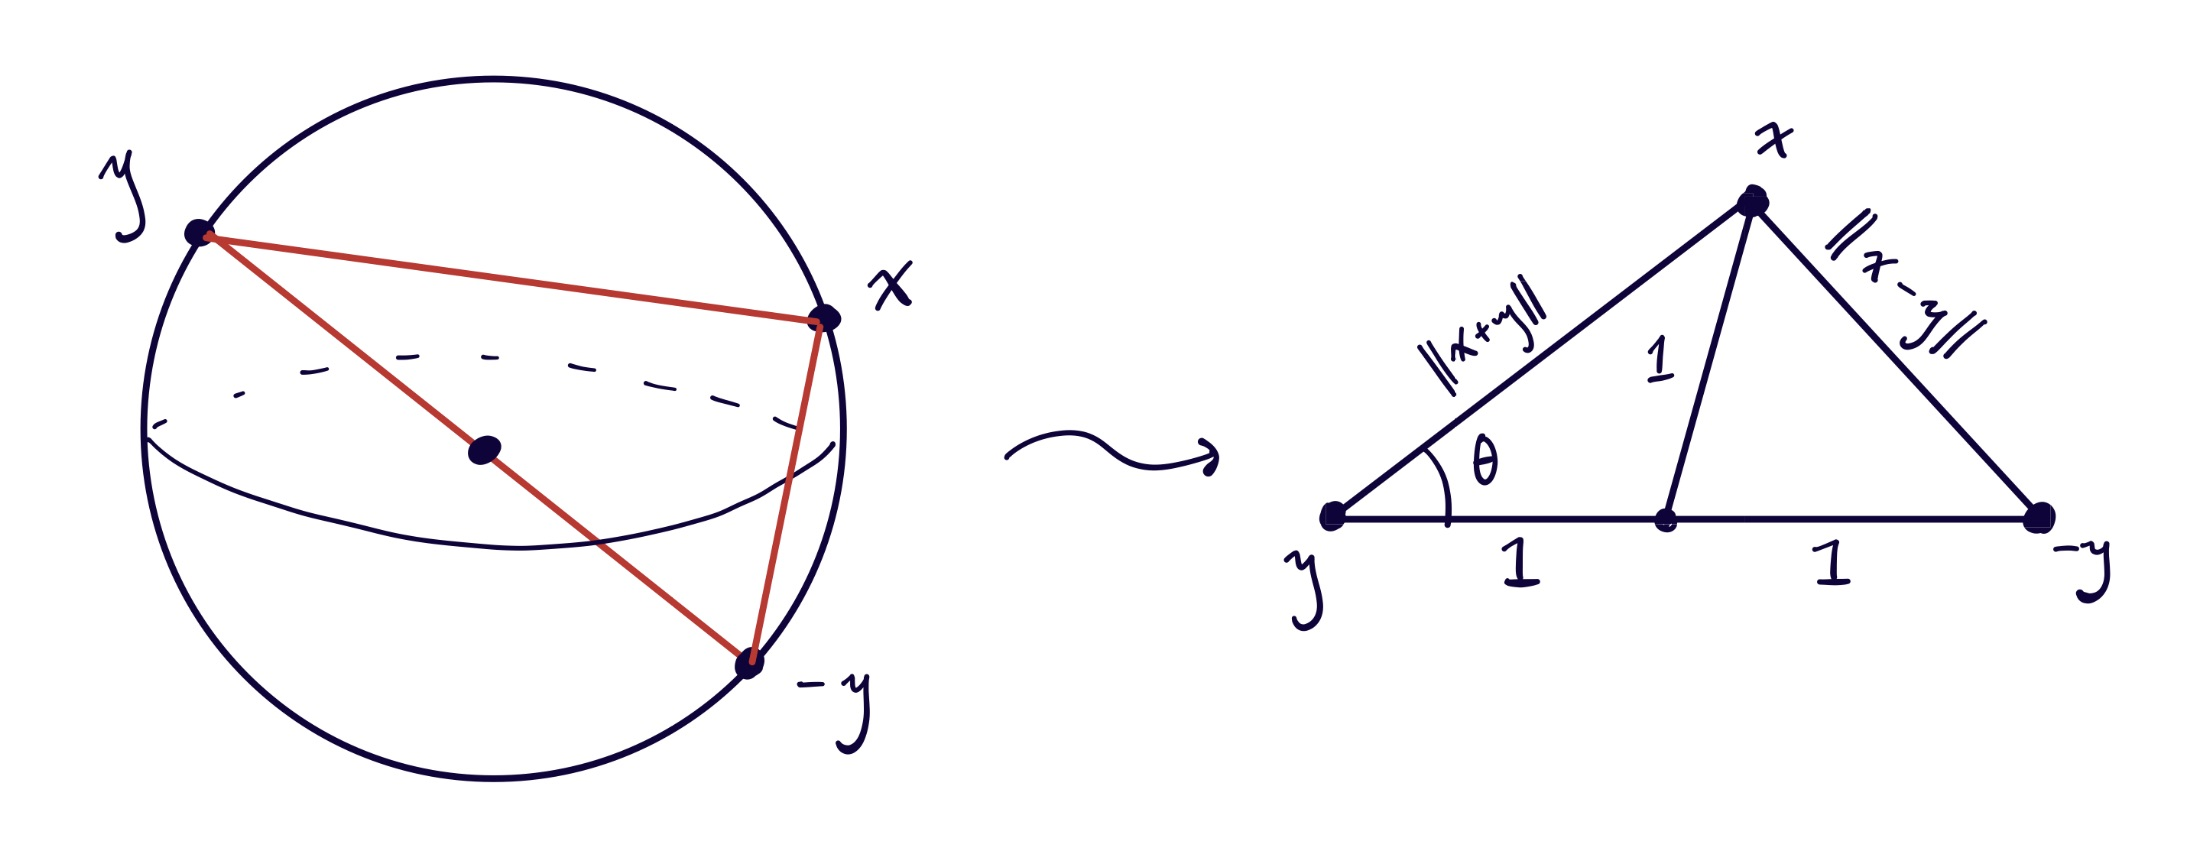
\includegraphics[width=12cm]{~/Desktop/university/latex/phd/data-sci/figures/hwk2-picture.png}
          \label{fig:prob2a}
          \captionof{figure}{The points $\bfx$ and $\bfy$ define a triangle}
        \end{center}
        Since $\|\bfx\|_2 = \|\bfy\|_2 = 1$, $x$ and $y$ lie on the unit sphere in $\bR^d$, and the sum $\|\bfx + \bfy\|_2 + \|\bfx - \bfy\|_2$ can be thought of as a portion of the perimeter of the triangle in Figure (2). This perimeter is maximized when $\theta = \pi/4$, in which case $\|\bfx+\bfy\| = \|\bfx - \bfy\| = \sqrt{2}$. Because
        \begin{align*}
          \|\bfx + \bfy\|^2_2 + \|\bfx - \bfy\|^2_2 = (\|\bfx + \bfy\| + \|\bfx - \bfy\|)^2 - 2\|\bfx + \bfy\|\|\bfx - \bfy\|,
        \end{align*}
        one can show that $\|\bfx + \bfy\|^2_2 + \|\bfx - \bfy\|^2_2$ attains a maximum value on the unit sphere whenever either $\|\bfx + \bfy\| + \|\bfx - \bfy\|$ is maximized or when $\bfx = \bfy$. In either case, $\|\bfx + \bfy\|^2_2 + \|\bfx - \bfy\|^2_2 = 4$.

        Combining this fact with the inequality above, we get that
        \begin{align*} 
          -4\epsilon &\leq -\epsilon(\|\bfx + \bfy\|^2_2 + \|\bfx - \bfy\|^2_2) \\
          &\leq \|\bfx + \bfy\|^2_2 - \|\bfx - \bfy\|_2^2 - (\|\Phi(x + y)\|^2_2 - \|\Phi(x - y)\|^2_2)\\
          &\leq \epsilon(\|\bfx + \bfy\|^2_2 + \|\bfx - \bfy\|^2_2) \leq 4\epsilon,
        \end{align*}
        or cutting out the 2nd and 4th terms,
        \begin{align*}
          -4\epsilon \leq \|\bfx + \bfy\|^2_2 - \|\bfx - \bfy\|_2^2 - (\|\Phi(x + y)\|^2_2 - \|\Phi(x - y)\|^2_2)\leq 4\epsilon.
        \end{align*}
        We can now use the linearity of $\Phi$ together with the given identity to see
        \begin{align*}
          -4 \epsilon \leq 4\langle \bfx,\bfy \rangle - 4\langle \Phi(\bfx),\Phi(\bfy) \rangle \leq 4\epsilon,
        \end{align*}
        and so we have
        \begin{align*}
          \big|\langle \bfx,\bfy \rangle - \langle \Phi(\bfx),\Phi(\bfy) \rangle\big| \leq \epsilon = \epsilon\|\bfx\|_2\|\bfy\|_2
        \end{align*}
        as desired.
      \item Denote by $\hat{\bfx} = \frac{\bfx}{\|\bfx\|}$ the normalization of a vector $\bfx\in \bR^d$. By the bilinearity of the inner product and the linearity of $\Phi$, we can factor out the product of norms:
        \begin{align*} 
          \big|\langle \bfx,\bfy \rangle - \langle \Phi(\bfx),\Phi(\bfy) \rangle\big| 
            &= \big|\langle ~ \|\bfx\|\cdot \hat{\bfx},\|\bfy\|\cdot \hat{\bfy} ~\rangle - \langle ~\Phi(\|\bfx\|\cdot \hat{\bfx}),\Phi(\|\bfy\|\cdot \hat{\bfy}) ~\rangle\big|\\
            &= \|\bfx\|\|\bfy\|\cdot \big|\langle \bfx,\bfy \rangle - \langle \Phi(\bfx),\Phi(\bfy) \rangle\big|,
        \end{align*}
        and after dividing out this product of norms and squaring, we get the result from part (a):
        \begin{align*}
          |\langle \bfx_j,\bfx_k \rangle - \langle \Phi(\bfx_j),\Phi(\bfx_k) \rangle| \leq \epsilon \|\bfx_j\|_2\|\bfx_k\|_2 \iff 
          |\langle \hat{\bfx}_j,\hat{\bfx}_k \rangle - \langle \Phi(\hat{\bfx}_j),\Phi(\hat{\bfx}_k) \rangle|^2 \leq \|\hat{\bfx}_j\|_2\|\hat{\bfx}_k\|_2^2.
        \end{align*}
        The matrix $\Phi$ precisely satisfies the hypotheses of the Johnson-Lindenstrauss Lemma, which means that
        \begin{align*}
          (1 - \epsilon)\|\bfx_j - \bfx_k\| \leq \|\Phi(\bfx_j) - \Phi(\bfx_k)\| \leq (1 + \epsilon)\|\bfx_j - \bfx_k\|
        \end{align*}
        occurs with probability at least $1 - \delta$ whenever $r \geq c\cdot \epsilon^{-2}\log(n/\delta)$. This is one of our hypotheses in part (a); to get the second one, we can expand our set $\chi$ by taking its union with $-\chi$:
        \begin{align*}
          \chi' = \chi \cup (-1)\cdot \chi = \{\bfx_1,...,\bfx_n,-\bfx_1,...,-\bfx_n\}.
        \end{align*}
        At worst, $\chi'$ has twice as many elements as $\chi$, so
        \begin{align*}
          (1 - \epsilon)\|\bfx_j \pm \bfx_k\| \leq \|\Phi(\bfx_j) \pm \Phi(\bfx_k)\| \leq (1 + \epsilon)\|\bfx_j \pm \bfx_k\|
        \end{align*}
        occurs with probability at least $1 - \delta$ whenever $r \geq c\cdot \epsilon^{-2}\log(2n/\delta)$ (notice the coefficient $2$ attached to $n$). Thus, by part (a), we get that  
        \begin{align*}
          |\langle \bfx_j,\bfx_k \rangle - \langle \Phi(\bfx_j),\Phi(\bfx_k) \rangle| \leq \epsilon \|\bfx_j\|_2\|\bfx_k\|_2.
        \end{align*}
        holds with probability at least $0.9$ whenever
        \begin{align*}
          r\geq c\dot \epsilon^{-2}\log(2n/0.1) = \frac{c\log(20n)}{\epsilon^2}.
        \end{align*}
    \end{enumerate}
  \end{prf}
  \prob Let $A$ be a square $n\times n$ matrix whose rows are orthonormal. Prove that the columns of $A$ are also orthonormal.
  \begin{prf}
    Since the rows of $A$ are orthonormal, we have that
    \begin{align*}
      [A\cdot A^\top]_{ij} = A_{i*}\cdot (A^T)_{*j} = A_{i*} \cdot A_{j*} =
      \begin{cases}
        1 & i = j\\
        0 & \text{else}
      \end{cases}
    \end{align*}
    where $A_{i*}$ and $(A^\top)_{*j}$ denote the $i$th row and $j$th column of $A$ and $A^\top$ respectively. This then implies that $A\cdot A^\top = I_n$. Because the left and right inverse of an invertible square matrix are the same, $A^\top \cdot A = I_n$ as well and by a calculation similar to the one above we get that 
    \begin{align*}
      (A^\top)_{i*}\cdot A_{*j} = A_{*i}\cdot A_{*j} =
      \begin{cases}
        1 & i = j \\
        0 & \text{else}
      \end{cases}.
    \end{align*}
    Hence, the columns of $A$ are also orthonormal.
  \end{prf}
  \prob Let $A$ be a square invertible matrix with SVD $\sum_i \sigma_i u_i v_i^\top$. Show that the inverse of $A$ is $\sum_i \sigma_i^{-1}v_i u_i^\top$.
  \begin{prf}
    Note first the because $A$ is invertible it has full rank equal to $n$, and hence has $n$ left and right singular vectors. Multiplying the proposed SVD of $A^{-1}$ with the SVD of $A$ gives us
    \begin{align*}
      \left(\sum_i \sigma_i u_i v_i^\top\right)\left(\sum_j \sigma_j^{-1}v_j u_j^\top\right) 
      &= \sum_i \left(\sigma_i u_iv_i^\top\cdot \sum_j\sigma^{-1}_jv_ju_j^{\top}\right)\\
      &= \sum_i\sum_j \sigma_i\sigma_j^{-1}(u_iv_i^\top v_ju_j^\top) \\
      &= \sum_i u_iu_i^{\top},
    \end{align*}
  where all sums range from $1,...,n$ implicitly. I'm told that one can directly show that the entries of $\sum_i u_iu_i^{\top}$ give the $n\times n$ identity matrix, but here is a slightly less tedious way to see this. By orthogonality of the $u_i$, we get that
  \begin{align*}
    \left(\sum_i u_iu_i^{\top}\right) u_j = u_j
  \end{align*}
  for any $1\leq j \leq n$. Since the $\{u_1,...,u_n\}$ vectors span are linearly independent, they span $\bR^n$ and we can therefore write any other vector $w \in \bR^n$ as a linear combination of the $u_i$. This implies
  \begin{align*}
    \left(\sum_i u_iu_i^{\top}\right) w = w.
  \end{align*}
  Lemma 3.3 in the text says that two matrices $A$ and $B$ are equal if and only if for every vector $\bfv$ $A\bfv = B\bfv$, and so by this lemma we conclude that $\sum_i u_iu_i^{\top} = I_n$.

  \bigskip
  
  Because the left and right inverses of invertible square matrices are equal and inverses of square matrices are unique, $A^{-1} = \sum_i \sigma_i^{-1}v_iu^{\top}$. In matrix notation, we would write
  \begin{align*}
    A^{-1} = V\Sigma^{-1} U^\top.
  \end{align*}
  \end{prf}
  \prob Let $\sum_{i=1}^r \sigma_i\bfu_i\bfv_i^\top$ be an SVD of a rank $r$ matrix $\bfA \in \bR^{m\times n}$ where $\sigma_1\geq \sigma_2\geq ...\geq \sigma_r$. Let $\bfA_k = \bR^{m\times n} = \sum_{i=1}^k \sigma_i\bfu_i\bfv_i^\top$ be the rank k approximation to $\bfA$ obtained by truncating its SVD. Express the following quantities in terms of the singular values $\{\sigma_i\}_{i=1}^r$:
  \begin{enumerate}[(i)]
    \item $\|\bfA\|_F^2$
    \item $\|\bfA\|_2^2$
    \item $\|\bfA - \bfA_k\|^2_F$
    \item $\|\bfA - \bfA_k\|_2^2$.
  \end{enumerate}
  \begin{prf}
    $ $
    \begin{enumerate}[(i)]
      \item Recall that the Frobenius norm of $\bfA$ is simply the standard Euclidean norm of $\bfA$ when considered to be a vector in $\bR^{m\times n}$, i.e.
        \begin{align*}
          \|\bfA\|_F^2 = \sum_{i=1}^m\sum_{j=1}^n [\bfA_{ij}]^2.
        \end{align*}
        As written, we are adding the squared norms of each row vector in $\bfA$. The squared norm of the $i$th row of $\bfA$ is the $i$th diagonal element of $\bfA\cdot\bfA^\top$, hence
        \begin{align*}
          \|\bfA\|_F^2 = \Tr(\bfA\cdot \bfA^\top).
        \end{align*}
        This formulation of the Frobenius norm makes it clear (after distributing products and using the pairwise orthogonality of the $\bfv_i$ a few times) that
        \begin{align*}
          \|\bfA\|_F^2 
            &= \Tr\left(\sum_{i=1}^r \sigma_i\bfu_i\bfv_i^\top \cdot \left(\sum_{i=1}^r \sigma_j\bfu_j\bfv_j^\top\right)^\top\right) \\
            &= \Tr\left(\sum_{i=1}^r \sigma_i\bfu_i\bfv_i^\top ~ \cdot ~ \sum_{i=1}^r \sigma_j\bfv_j\bfu_j^\top\cdot \right) \\
            &= \Tr\left(\sum_{i=1}^r \sigma_i^2 e_i\right) \\
            &= \sigma^2_1 + ... + \sigma^2_r
        \end{align*}
      \item The spectral norm of $\bfA$ is defined
        \begin{align*}
          \|\bfA\|_2^2 = \max_{\substack{v \in \bR^n\\\|v\| = 1}} \left|A v\right|.
        \end{align*}
        The right singular vector $\bfv_1$ of $\bfA$ is, by definition, the norm 1 vector which maximizes $\left|Av\right|$, and $\sigma_1$ is this value. Hence,
        \begin{align*}
          \|\bfA\|_2^2 = \sigma_1.
        \end{align*}
      \item The matrix $\bfA - \bfA_k$ is a matrix whose SVD is given by $\sum_{i=k+1}^r \sigma_i \bfu_i\bfv_i^\top$. Hence, by part \emph{(i)},
        \begin{align*}
          \|\bfA - \bfA_k\|_F^2 = \sigma_{k+1}^2 + ... + \sigma_r^2.
        \end{align*}
      \item Similarly, by part \emph{(ii)},
        \begin{align*}
          \|\bfA - \bfA_k\|_2^2 = \sigma_{k+1}
        \end{align*}
        because $\bfA - \bfA_k$ is a matrix whose SVD is given by $\sum_{i=k+1}^r \sigma_i\bfu_i\bfv_i^\top$.
    \end{enumerate}
  \end{prf}
  \prob $ $
  \begin{enumerate}[(a)]
    \item Write a program to implement the power method for computing the first right singular vector of a matrix. Apply your program to the matrix
      \begin{align*}
        A = 
        \begin{pmatrix}
          1 & 2 & 3 & \dots & 9 & 10 \\
          2 & 3 & 4 & \dots & 10 & 0 \\
          \vdots & \vdots & \vdots & & \vdots & \vdots \\
          9 & 10 & 0 & \dots & 0 & 0 \\
          10 & 0 & 0 & \dots & 0 & 0 
        \end{pmatrix}.
      \end{align*}
      \item Implement a modification of the power method that computes the first four right singular vectors of a matrix, as follows. Randomly select four vectors and find an orthonormal basis for the space spanned by the four vectors. Then multiply each of the basis vectors by $\bfA\bfA^\top$ and find a new orthonormal basis for the space spanned by the resulting four vectors. Apply your code to compute the first four singular vectors of the matrix from part (a). Comment on how you might extend this to compute the first $k$ singular vectors of a matrix.
  \end{enumerate}
  \begin{soln}$ $
    \begin{enumerate}[(a)]
      \item Numerical precision poses a problem here, and I actually had better results after implementing this in Rust as it forces you to specify types. Python matched the precision once I told numpy to use float64. The attached python program estimated that the first left singular vector of $A$ was
        \begin{align*} \bfu_1 = 
          \begin{bmatrix}
            -0.3197506\\
            -0.36962502\\
            -0.39811309\\
            -0.4039189\\
            -0.38728043\\
            -0.3499587\\
            -0.29512626\\
            -0.22716238\\
            -0.15136864\\
            -0.07362363
          \end{bmatrix} 
        \end{align*}
        by taking the first column of $(A\cdot A^\top)^{16}$ and normalizing. This had an error of $8.007677*10^{-9}$ when compared with the first left singular vector given by the numpy.linalg.svd function. The sign of the elements in the estimate $\hat{\bfu_1}$ for $\bfu_1$ is manually set to match that of the singular vector calculated by numpy, to ensure the error is accurate. Note that because $A$ is symmetric, the $i$th left and right singular vectors are the same.

      \item The relevant code for this portion is contained in the function problem6b(). We first generate four random vectors from a standard Gaussian distribution on $\bR^{10}$. We then perform QR-factorization to find an orthonormal basis for the subspace spanned by these vectors and calculate the product
        \begin{align*}
          A\cdot A^\top \cdot Q
        \end{align*}
        from right to left. This is equivalent to calculating the individual matrix-vector products for the column vectors of $Q$ individually. To get a better estimate, we iterate this process: perform QR-factorization on $A\cdot A^\top \cdot Q$ to obtain $Q_1$ and then find $A\cdot A^T \cdot Q_1$. We did this 16 times, in order to match the iterations in part (a). Finally, we compare the result to numpy.linalg.svd and examine the error. I won't print the estimates for the first four singular vectors of $A$ here; instead, I'll list the errors:
        \begin{align*}
          \bfu_1&: ~ \text{ error on the order of } 10^{-9} \\
          \bfu_2&: ~ \text{ error on the order of } 10^{-8} \\
          \bfu_3&: ~ \text{ error on the order of } 10^{-5} \\
          \bfu_4&: ~ \text{ error on the order of } 10^{-4}. \\
        \end{align*}
        It is once again likely that the error grows as the singular vectors become less significant due to some numerical precision errors.

        We could generalize this process to find the first $k$ left singular vectors by first generating $k$ random vectors rather than $4$. It is important that we reorthonormalize each time we apply $A\cdot A^\top$ to $Q$ in order to ensure the first singular vector doesn't begin to dominate. Here is an image of my code output for this portion of the problem:
      \begin{center}
        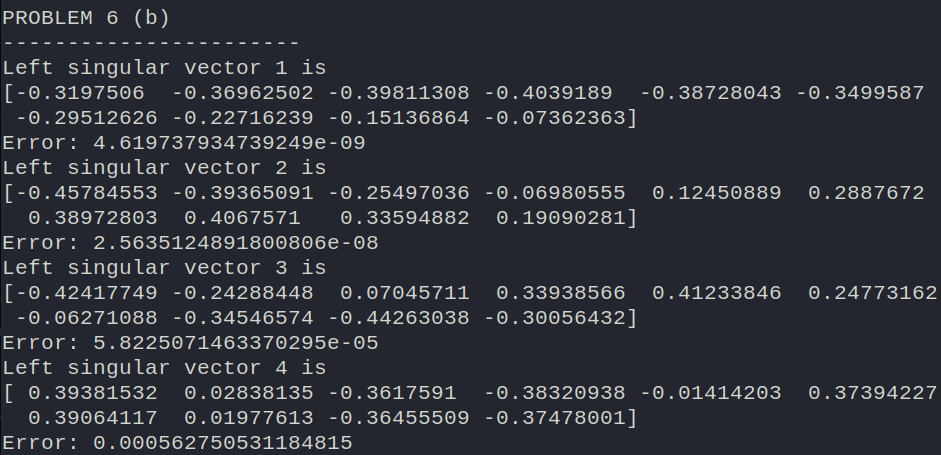
\includegraphics[width=12cm]{~/Desktop/university/latex/phd/data-sci/figures/hwk2-terminal-output.png}
        \label{fig:prob6b}
      \end{center}
    \end{enumerate}
  \end{soln}
  \prob Read in a grayscale image of your choice, or resolution at least 256 by 256. Perform a singular value decomposition of the matrix. Reconstruct the image using only the 1, 4, 16 and 32 singular values/singular vectors.
  \begin{enumerate}[(a)]
    \item Plot the original image along with the reconstructed images.
    \item What percentage of the Frobenius norm is captured in each case?
    \item Repeat steps (a) and (b) above, but now for a ``white noise'' image of the same dimensions generated as follows: each pixel is generated as an independent uniform random variable on $[0,1]$. Compare the behavior of the singular values for the noise image and the real image. Please discuss.
  \end{enumerate}
  \begin{soln}$ $
    \begin{enumerate}[(a)]
      \item I plotted this for two images, one a $600 \times 600$ image of a rock and another a $900 \times 900$ painting of a waterfall (it looks a lot like Yosemite falls to me). Here are the results.
      \begin{center}
        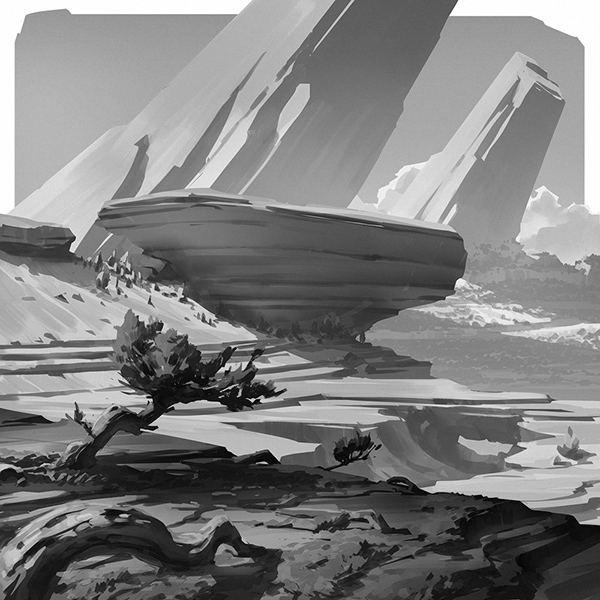
\includegraphics[width=12cm]{~/Desktop/university/code/dsml/hwk2/images/bwrock.jpg}
        \captionof{figure}{Original image}
        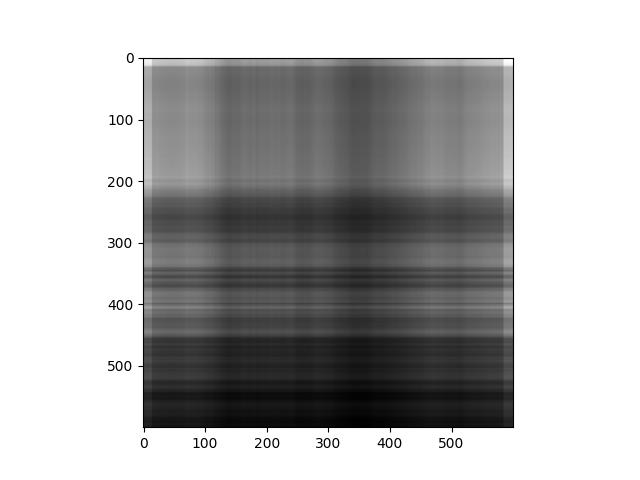
\includegraphics[width=12cm]{~/Desktop/university/code/dsml/hwk2/images/bwrock1.jpg}
        \captionof{figure}{Image reconstructed with 1 singular value, captured 95.258\% of the Frobenius norm}
        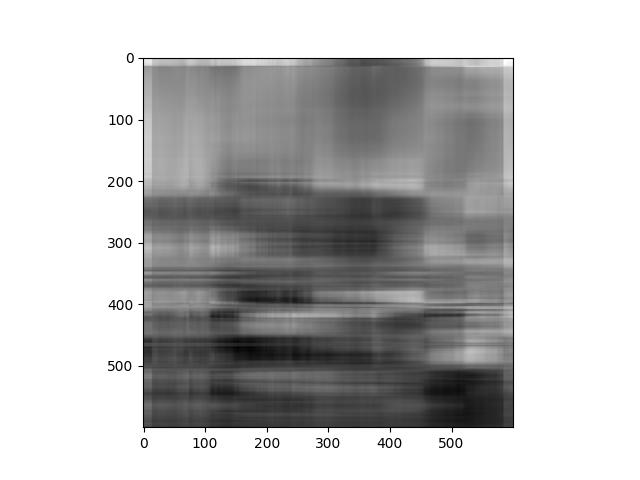
\includegraphics[width=12cm]{~/Desktop/university/code/dsml/hwk2/images/bwrock4.jpg}
        \captionof{figure}{Image reconstructed with 4 singular values, captured 97.421\% of the Frobenius norm}
        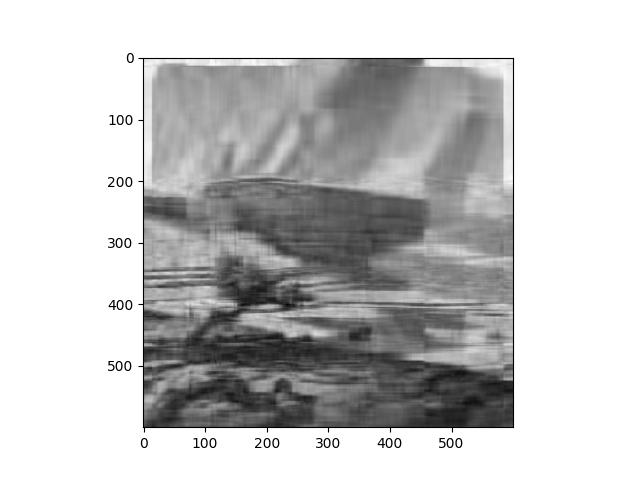
\includegraphics[width=12cm]{~/Desktop/university/code/dsml/hwk2/images/bwrock16.jpg}
        \captionof{figure}{Image reconstructed with 16 singular values, captured 99.060\% of the Frobenius norm}
        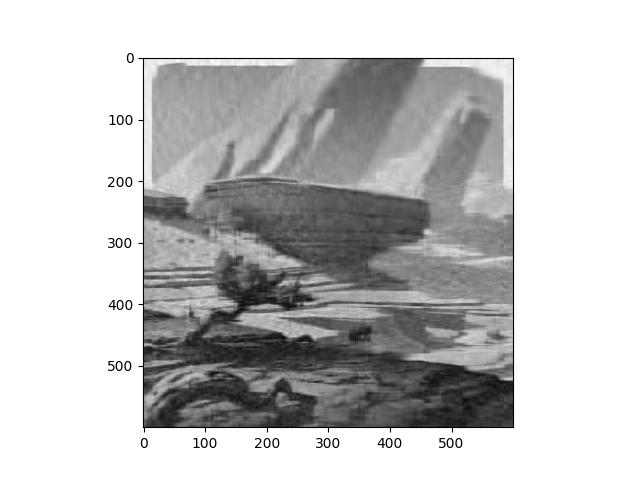
\includegraphics[width=12cm]{~/Desktop/university/code/dsml/hwk2/images/bwrock32.jpg}
        \captionof{figure}{Image reconstructed with 32 singular values, captured 99.464\% of the Frobenius norm}
        \label{fig:prob7a1}
      \end{center}
      \begin{center}
        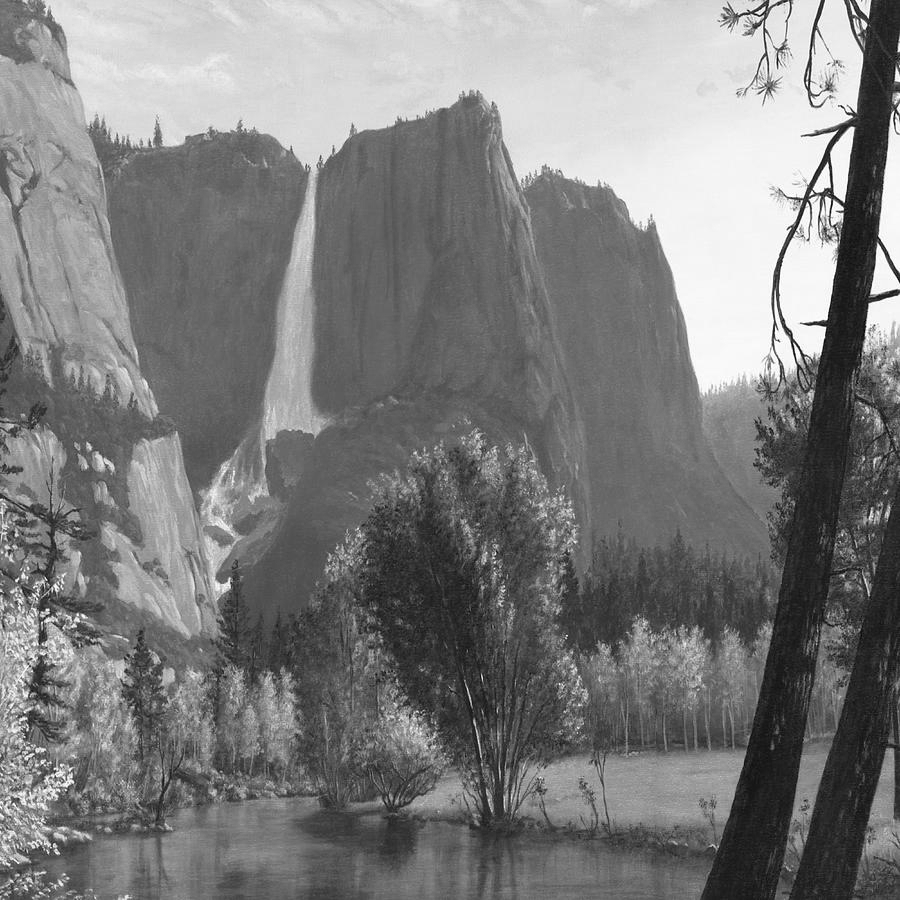
\includegraphics[width=12cm]{~/Desktop/university/code/dsml/hwk2/images/bwwaterfall.jpg}
        \captionof{figure}{Original image}
        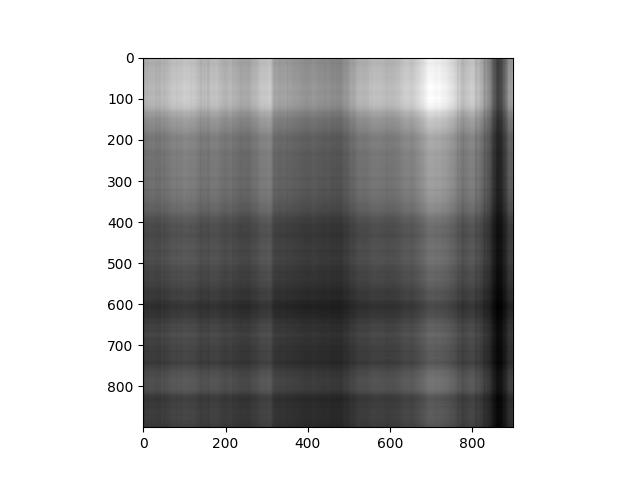
\includegraphics[width=12cm]{~/Desktop/university/code/dsml/hwk2/images/bwwaterfall1.jpg}
        \captionof{figure}{Image reconstructed with 1 singular value, captured 95.345\% of the Frobenius norm}
        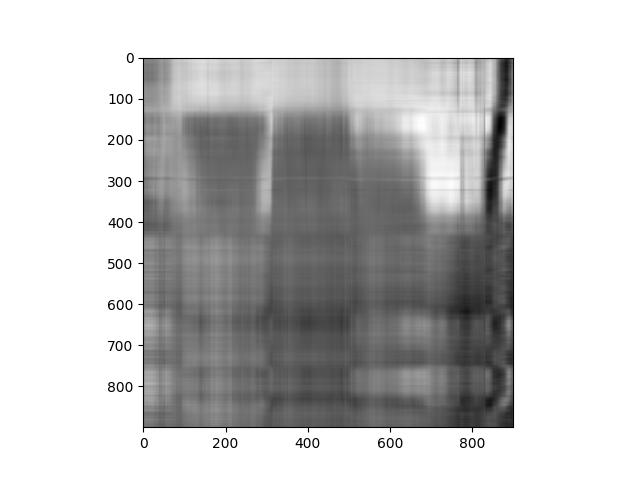
\includegraphics[width=12cm]{~/Desktop/university/code/dsml/hwk2/images/bwwaterfall4.jpg}
        \captionof{figure}{Image reconstructed with 4 singular values, captured 97.835\% of the Frobenius norm}
        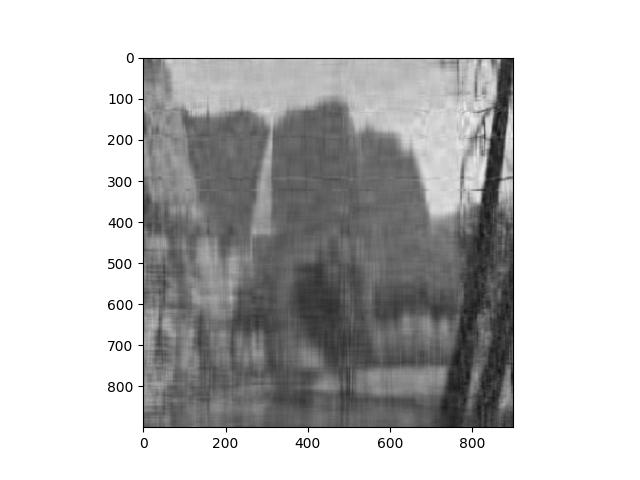
\includegraphics[width=12cm]{~/Desktop/university/code/dsml/hwk2/images/bwwaterfall16.jpg}
        \captionof{figure}{Image reconstructed with 16 singular values, captured 99.012\% of the Frobenius norm}
        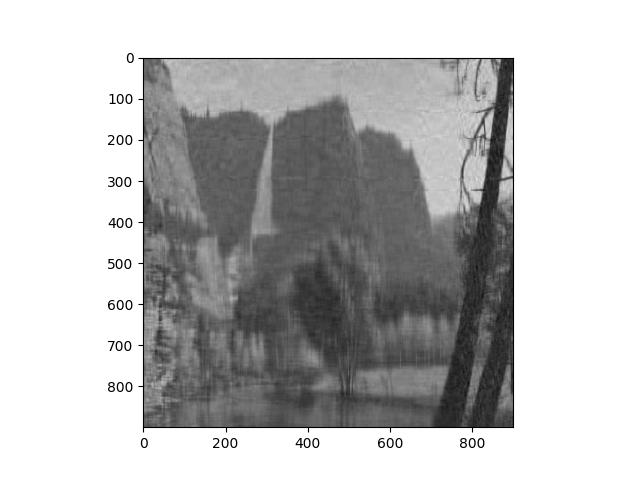
\includegraphics[width=12cm]{~/Desktop/university/code/dsml/hwk2/images/bwwaterfall32.jpg}
        \captionof{figure}{Image reconstructed with 32 singular values, captured 99.351\% of the Frobenius norm}
        \label{fig:prob7a2}
      \end{center}
      \item The percentage of the Frobenius norm captured in each case is listed in the image captions. However, within a small margin of error, in both cases the percentage of the Frobenius norm captured is 95.3\% for 1 singular value, 97.6\% for 4 singular values, 99.04\% for 16 singular values and 99.40\% for 32 singular values. At the very least, this illustrates that closeness in Frobenius norm is a poor measurement of human image recognition. I can't begin to discern details until at least 16 singular values have been incorporated, at which point the images are already 99\% similar.
      \item Here are the plots generated for a $600 \times 600$ image of random noise.
      \begin{center}
        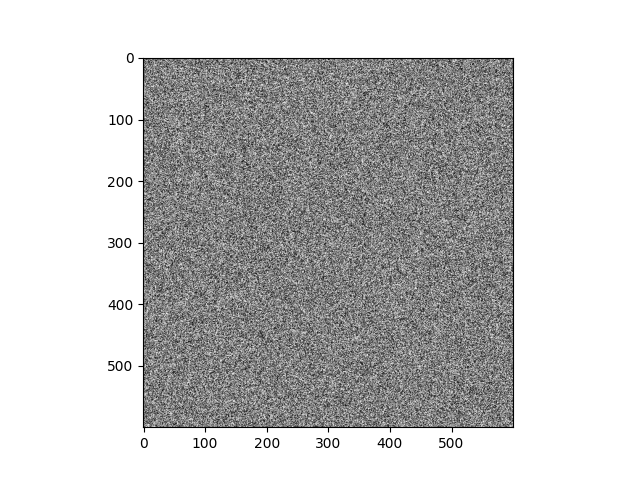
\includegraphics[width=12cm]{~/Desktop/university/code/dsml/hwk2/images/noise.png}
        \captionof{figure}{Original image}
        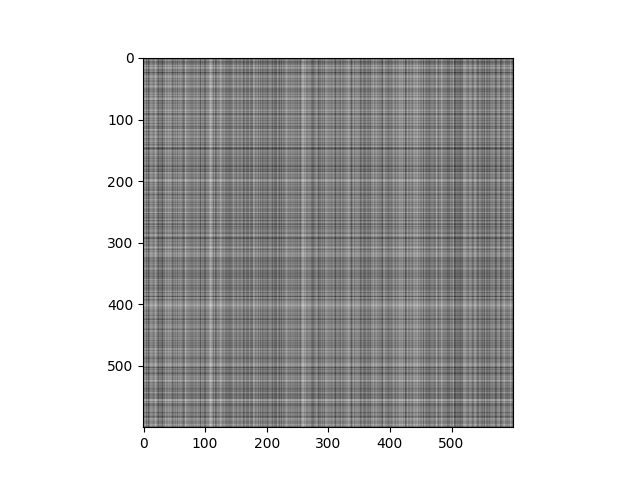
\includegraphics[width=12cm]{~/Desktop/university/code/dsml/hwk2/images/noise1.png}
        \captionof{figure}{Image reconstructed with 1 singular value, captured 86.646\% of the Frobenius norm}
        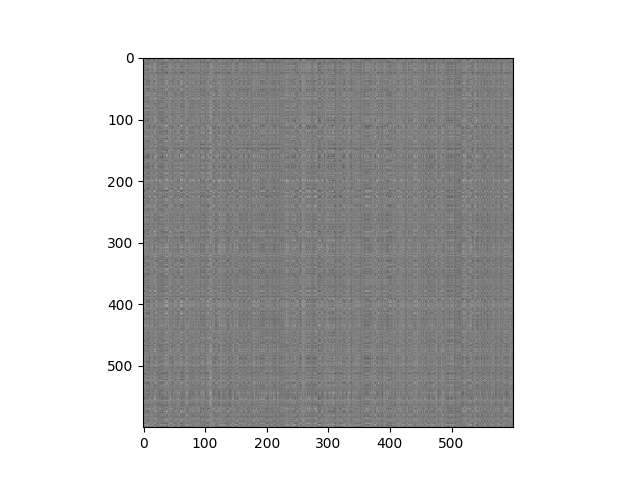
\includegraphics[width=12cm]{~/Desktop/university/code/dsml/hwk2/images/noise4.png}
        \captionof{figure}{Image reconstructed with 4 singular values, captured 86.925\% of the Frobenius norm}
        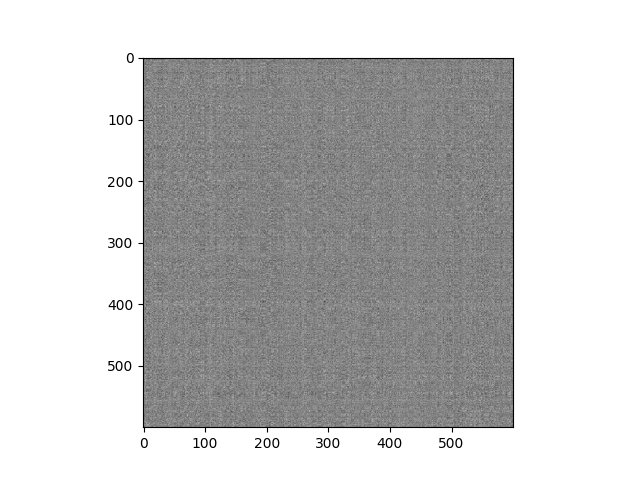
\includegraphics[width=12cm]{~/Desktop/university/code/dsml/hwk2/images/noise16.png}
        \captionof{figure}{Image reconstructed with 16 singular values, captured 87.945\% of the Frobenius norm}
        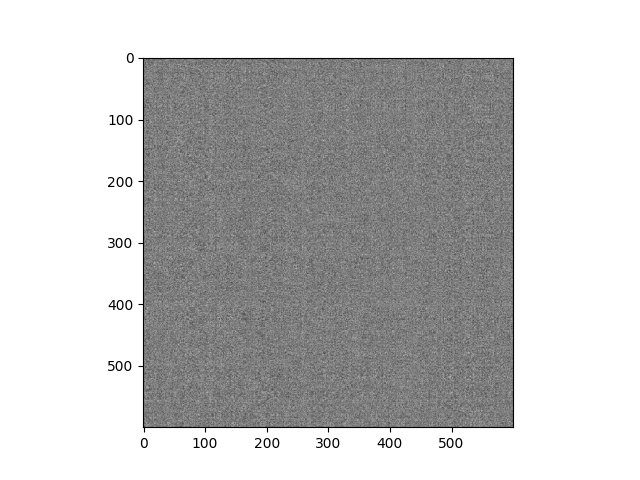
\includegraphics[width=12cm]{~/Desktop/university/code/dsml/hwk2/images/noise32.png}
        \captionof{figure}{Image reconstructed with 32 singular values, captured 89.155\% of the Frobenius norm}
        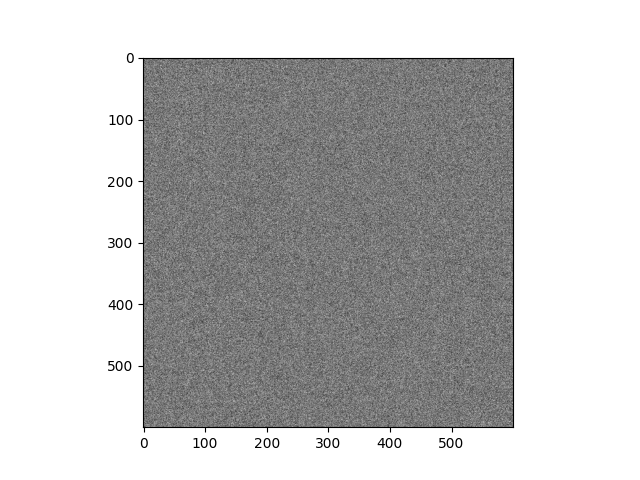
\includegraphics[width=12cm]{~/Desktop/university/code/dsml/hwk2/images/noise128.png}
        \captionof{figure}{Image reconstructed with 128 singular values, captured 94.324\% of the Frobenius norm}
        \label{fig:prob7c1}
      \end{center}
      The results show that it is far harder for SVD to compress a random image than a ``natural'' image. Human constructed images and photographs are more likely to have continuously varying color/brightness, i.e. the color of nearby neighboring pixels is likely to match within some margin of error. Loosely, this should mean that regional behavior of the image should capture something about the individual values of a pixel within that region. The image built from random noise features no such correlation between neighboring pixels. To approximate the behavior of an individual pixel, it is therefore necessary to read the value of the pixel itself.
    \end{enumerate}
  \end{soln}
\end{homework}
\end{document}
